\documentclass[12pt,xcolor=dvipsnames]{beamer}
\usecolortheme[named=Maroon]{structure}
\usetheme{Luebeck}
\usepackage[utf8]{inputenc}
\usepackage{amsmath}
\usepackage{amsfonts}
\usepackage{amssymb}
\usepackage{graphicx}
\usepackage{hyperref}
\DeclareMathOperator\erfc{erfc}
\graphicspath{{../plots/}}
\author{Jonathan Morrell, Tyler Bailey, Mitch Negus}
\title{HFNG Flux Calculation}
%\setbeamercovered{transparent} 
%\setbeamertemplate{navigation symbols}{} 
%\logo{} 
%\institute{} 
%\date{} 
%\subject{} 
\begin{document}

\begin{frame}
\titlepage
\end{frame}

\begin{frame}
\frametitle{Overview}
\begin{columns}[c]
\column{2in}
\begin{itemize}
\item Experiment summary
\item DD fusion spectrum
\item Solution method
\item Implementation
\item Results
\end{itemize}
\column{2in}
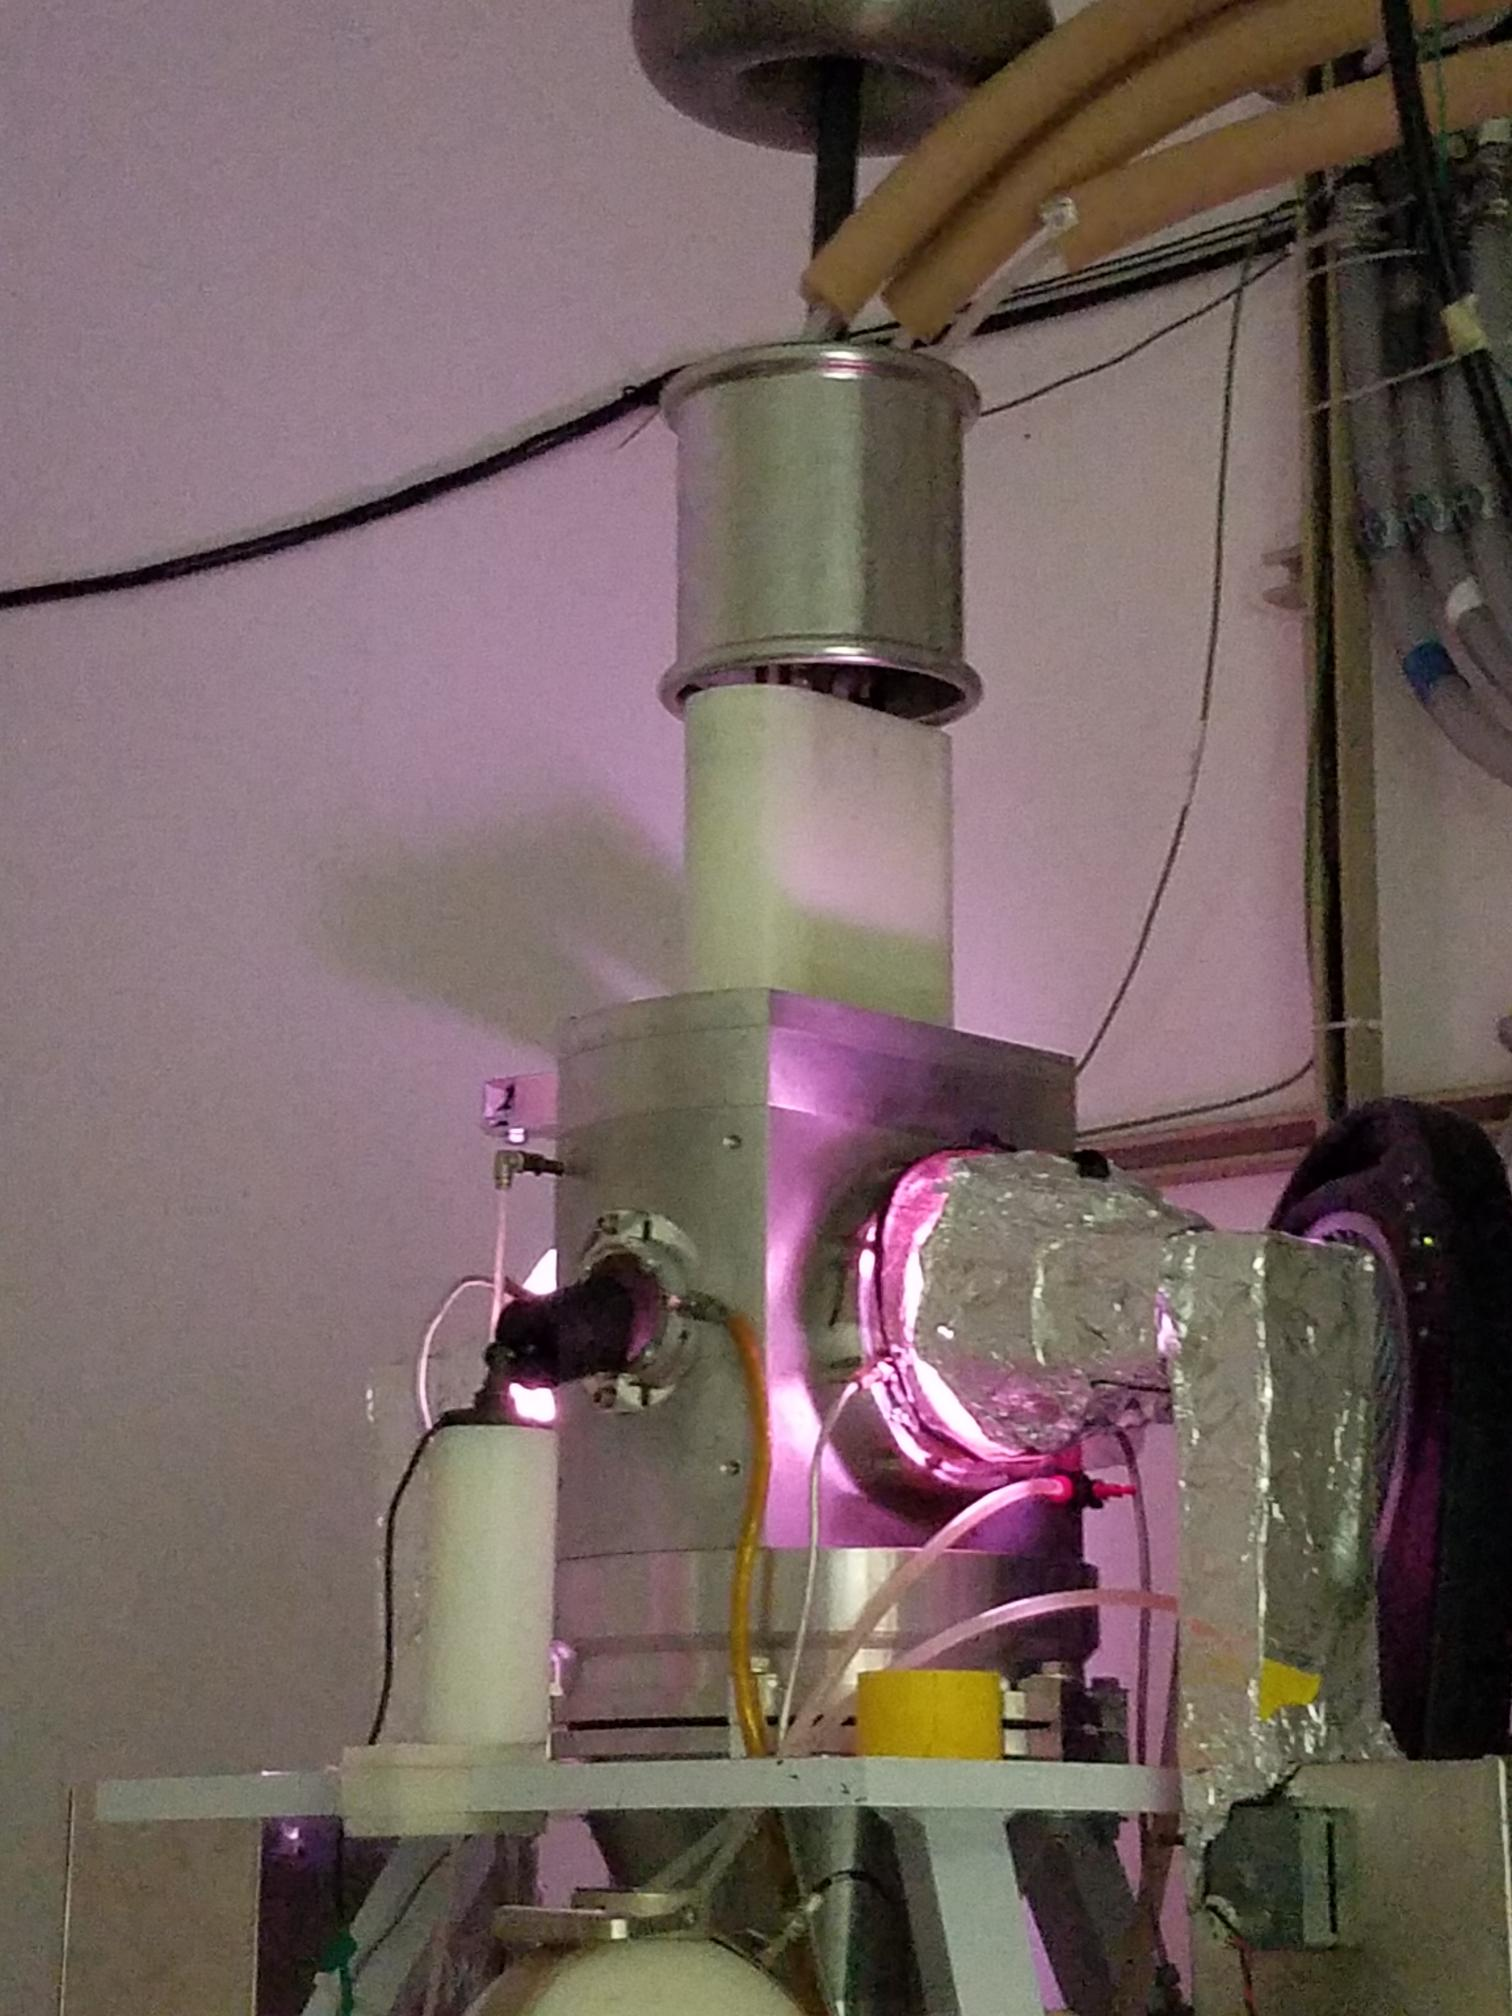
\includegraphics[width=2in]{hfng.jpg}
\end{columns}
\end{frame}


\begin{frame}
\frametitle{Experiment Summary}
\begin{columns}[c]
\column{2.5in}
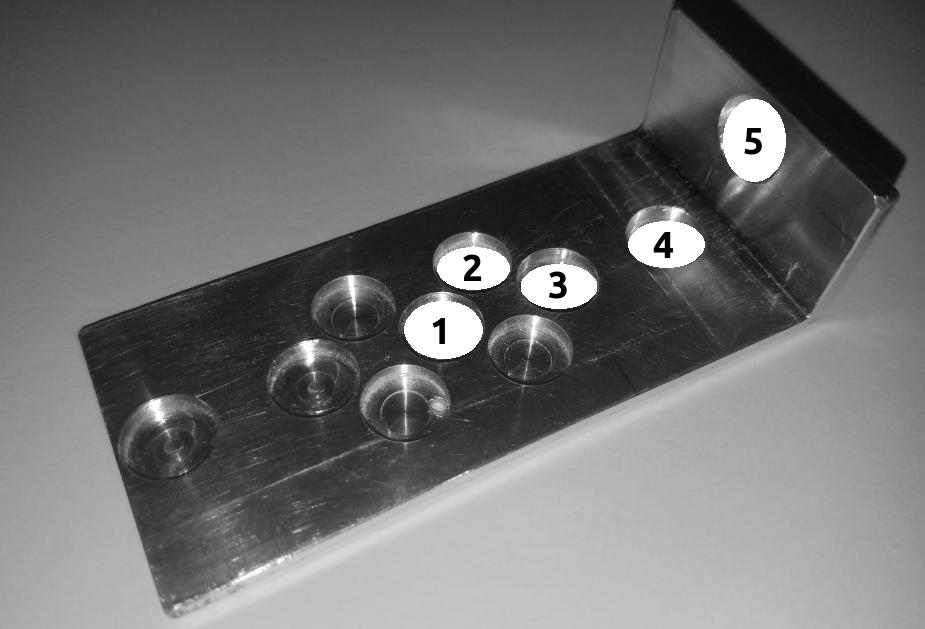
\includegraphics[width=2.5in]{sample_holder.jpg}
\column{1.5in}
\begin{itemize}
\item Goal to measure $^{35}$Cl(n,p)$^{35}$S cross section
\item 5x 11 mm OD NaCl pellets
\item Monitor fluence using $^{58}$Ni(n,p)$^{58}$Co
\item Need to determine energy spectrum for each sample
\end{itemize}
\end{columns}
\end{frame}


\begin{frame}
\frametitle{Experiment Summary}
\begin{center}
\begin{tabular}{c|cccc}
\hline 
Sample & $\Delta$x [mm] & $\Delta$y [mm] & $\Delta$z [mm] & $\Delta \theta$ [$^{\circ}$] \\ 
\hline 
1 & 0.0 & 0.0 & 8.0 & 0 \\ 
2 & 9.0 & 8.0 & 8.0 & 0 \\ 
3 & 18.0 & 0.0 & 8.0 & 0 \\ 
4 & 36.0 & 0.0 & 8.0 & 0 \\ 
5 & 46.0 & 0.0 & -7.0 & 90 \\ 
\hline 
\end{tabular}
\end{center}
\begin{columns}[c]
\column{1.5in}
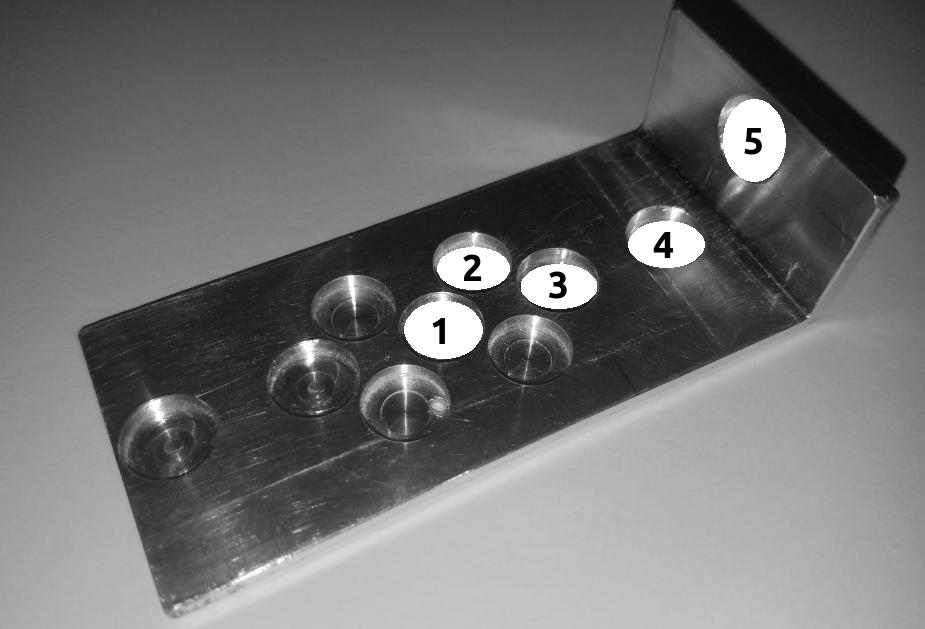
\includegraphics[width=1.5in]{sample_holder.jpg}
\column{2.5in}
\begin{itemize}
\item $\Delta$x, $\Delta$y, $\Delta$z relative to beam center
\item Additional 1.5 mm $\Delta$z due to thickness of sample holder
\item 14 mm beam diameter
\end{itemize}
\end{columns}
\end{frame}

\begin{frame}
\frametitle{DD Fusion Spectrum}
\begin{columns}[c]
\column{2in}
\begin{tabular}{c|cc}
\hline 
$A_n$ & 100 keV & 200 keV \\ 
\hline 
$A_0$ & 2.4674 & 2.47685 \\ 
$A_1$ & 0.30083 & 0.39111 \\ 
$A_2$ & 0.01368 & 0.04098 \\ 
$A_3$ & 0.0 & 0.02957 \\ 
\hline 
\end{tabular}\\
\ \ \\
$E_n(\theta) = A_0 + \sum_{n=1}^3 A_n cos^n(\theta)$
\column{2in}
\begin{tabular}{c|cc}
\hline 
$A_n$ & 100 keV & 200 keV \\ 
\hline 
$A_1$ & 0.01741 & -0.03149 \\ 
$A_2$ & 0.88746 & 1.11225 \\ 
$A_3$ & 0.22497 & 0.38659 \\
$A_4$ & 0.08183 & 0.26676 \\
$A_5$ & 0.37225 & 0.11518 \\ 
\hline 
\end{tabular}\\
\ \ \\
$\frac{R(\theta)}{R(90^{\circ})}=1+\sum_{n=1}^5 A_n cos^n(\theta)$
\end{columns}
\begin{itemize}
\item Use neutron energy and intensity correlations as input to source definition
\end{itemize}
\end{frame}

\begin{frame}
\frametitle{DD Fusion Spectrum}
\begin{columns}[c]
\column{2in}
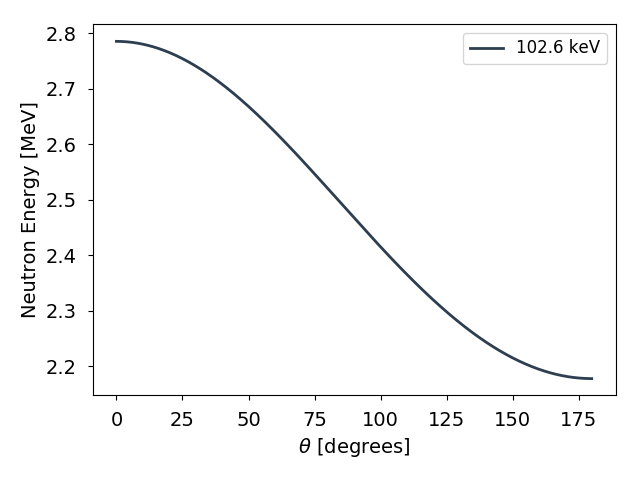
\includegraphics[width=2in]{energy_angle.png}\\
$E_n(\theta) = A_0 + \sum_{n=1}^3 A_n cos^n(\theta)$
\column{2in}
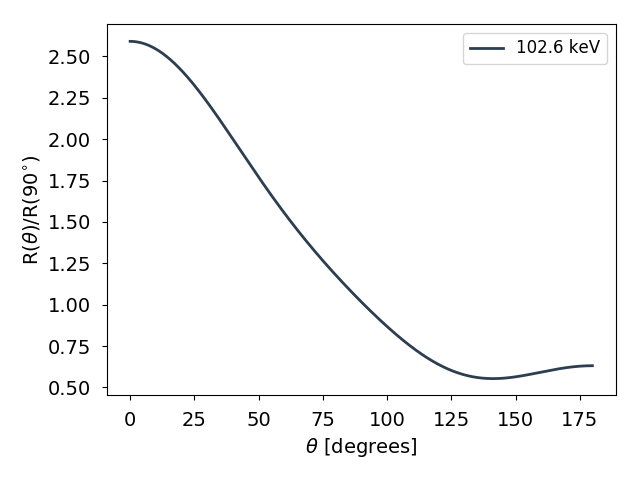
\includegraphics[width=2in]{intensity_angle.png}\\
$\frac{R(\theta)}{R(90^{\circ})}=1+\sum_{n=1}^5 A_n cos^n(\theta)$
\end{columns}
\begin{itemize}
\item Use neutron energy and intensity correlations as input to source definition
\end{itemize}
\end{frame}

\begin{frame}
\frametitle{Solution Method}
Solve for average flux over sample (in vacuum) for given source definition and sample geometry using Monte Carlo
\begin{align*}
\bar{\phi}(E) &= \int \int S(\vec{r},E,\hat{\Omega})d^3rd\hat{\Omega} \\
              &= \int \int \phi_0 \frac{n(\vec{r})\delta (\hat{\Omega}-\Omega_{sample})R(\theta(E))}{|\vec{r}-r|^2} d^3rd\hat{\Omega} \\
              &= \frac{1}{N} \sum_{n=1}^{N} \phi_0 \frac{R(\theta(E_n))\delta_{r\theta}}{(\Delta r_n)^2} = \phi_0 \sum_{n=1}^{N} \frac{R(\theta(E_n))\delta_{r\theta}}{(\Delta r_n)^2}
\end{align*}
where $n(\vec{r})$ is PDF for source (e.g. Gaussian) and $\delta_{r\theta}$ constrains neutron rays to source-sample paths. 
\end{frame}


\begin{frame}
\frametitle{Solution Method}
Generate ray coordinates by randomly generating source point from (radial) Gaussian distribution, and sample point from (radial) uniform distribution.\\
\ \ \\
\begin{columns}[c]
\column{2in}
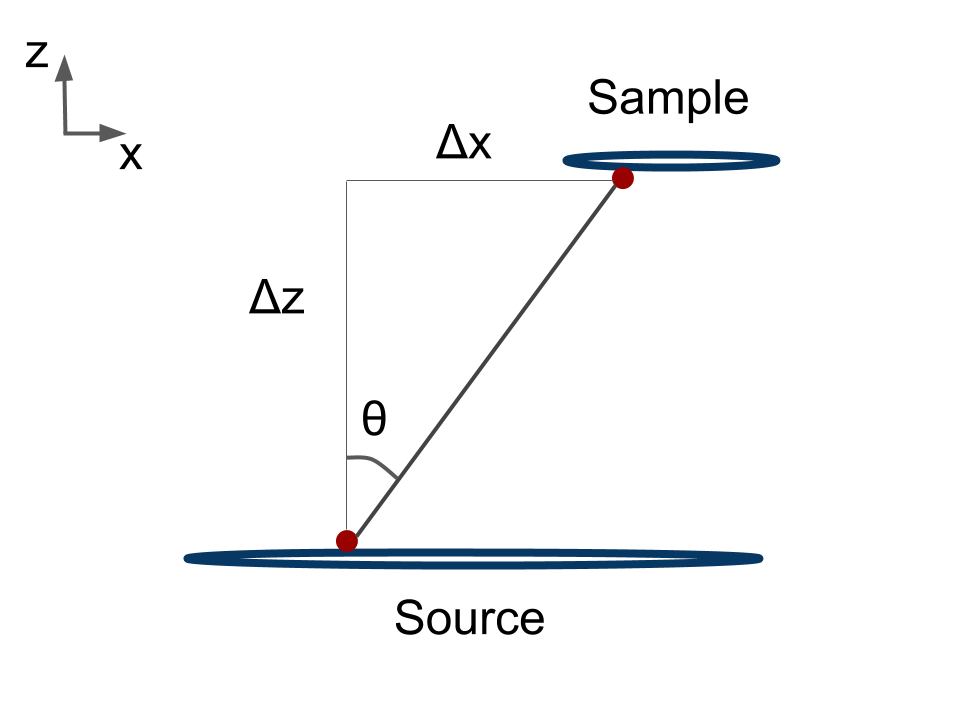
\includegraphics[width=2in]{MC201_Graphic.png}
\column{2in}
In general:\\
$\theta = arccos(\frac{\vec{r_1}\cdot\vec{r_2}}{|\vec{r_1}||\vec{r_2}|})$\\
\ \ \\
In 2D Cartesian:\\
$\theta = arccos(\frac{\Delta z}{\sqrt{\Delta x^2 + \Delta z^2}})$\\
\ \ \\
In 3D Cartesian:\\
$\theta = arccos(\frac{\Delta z}{\sqrt{\Delta x^2 + \Delta y^2 + \Delta z^2}})$\\
\ \ \\
\end{columns}
\end{frame}

\begin{frame}
\frametitle{Implementation}
\begin{columns}[c]
\column{2in}
\begin{itemize}
\item Implemented in python 2.7
\item Source on github:
\item \url{https://github.com/jtmorrell/MC_NE201}
\item Generates plots of flux spectrum for each sample and prints $E_{average}\pm 1\sigma_E$
\end{itemize}
\column{2in}
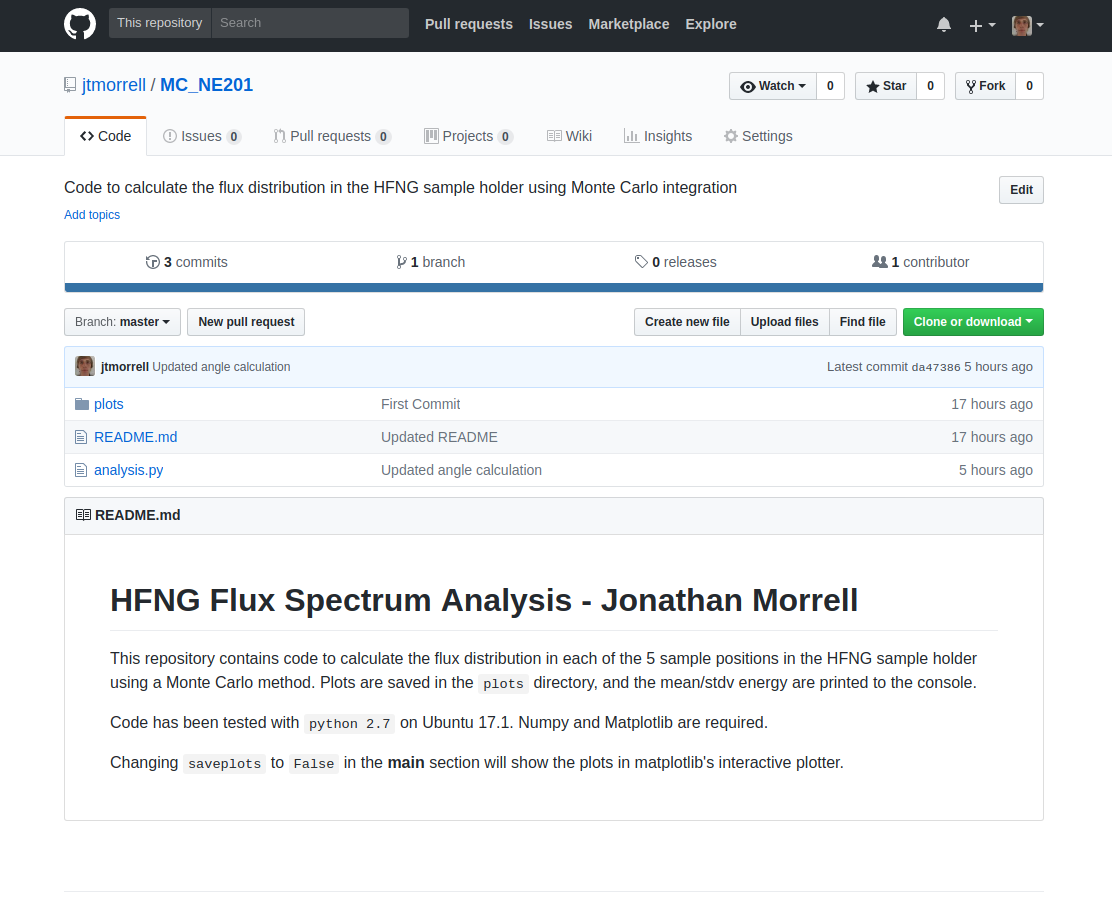
\includegraphics[width=2in]{github.png}
\end{columns}
\end{frame}

\begin{frame}
\frametitle{Results (Sample 1)}
\centering
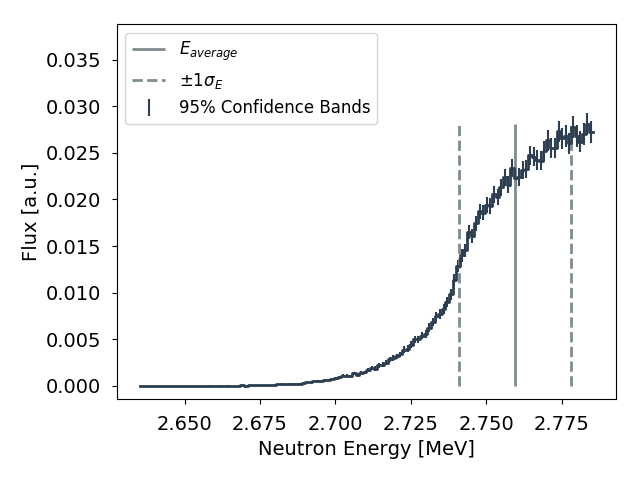
\includegraphics[width=3.5in]{009False.png}\\
$E_n=2.76\pm 0.019$ [MeV]
\end{frame}

\begin{frame}
\frametitle{Results (Sample 2)}
\centering
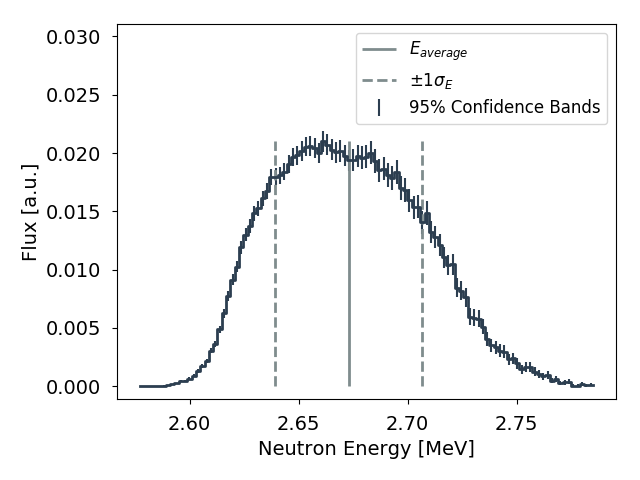
\includegraphics[width=3.5in]{989False.png}\\
$E_n=2.67\pm 0.033$ [MeV]
\end{frame}

\begin{frame}
\frametitle{Results (Sample 3)}
\centering
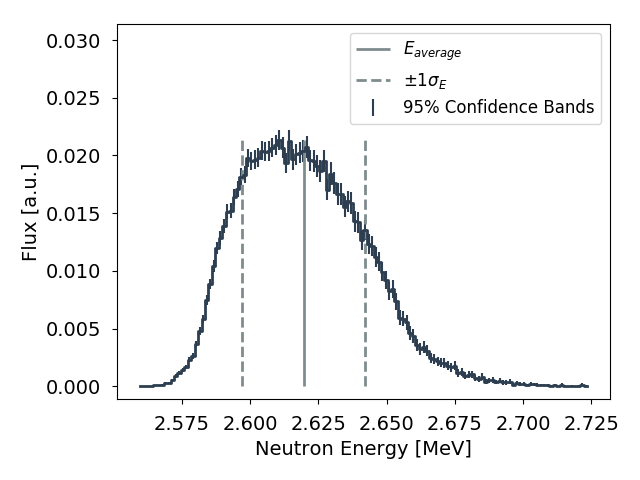
\includegraphics[width=3.5in]{1809False.png}\\
$E_n=2.62\pm 0.023$ [MeV]
\end{frame}

\begin{frame}
\frametitle{Results (Sample 4)}
\centering
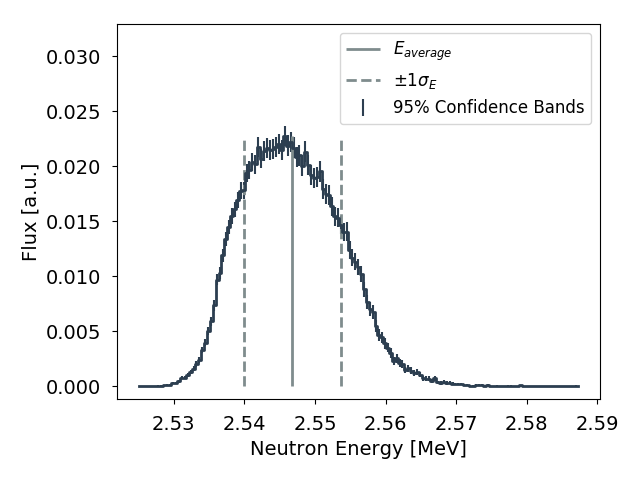
\includegraphics[width=3.5in]{3609False.png}\\
$E_n=2.55\pm 0.007$ [MeV]
\end{frame}

\begin{frame}
\frametitle{Results (Sample 5)}
\centering
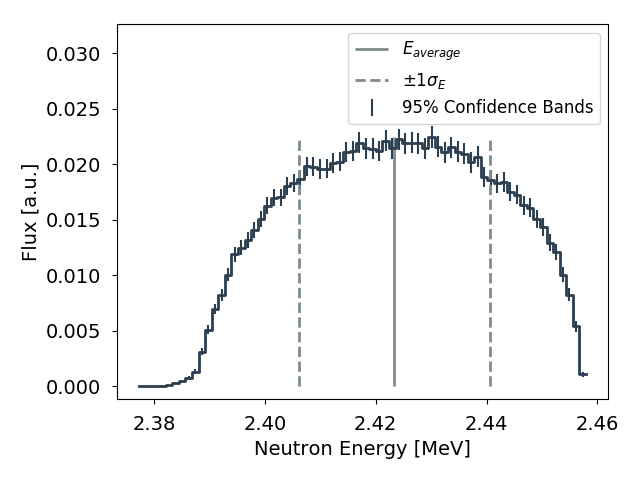
\includegraphics[width=3.5in]{-7046True.png}\\
$E_n=2.47\pm 0.018$ [MeV]
\end{frame}

\begin{frame}
\frametitle{Summary of Results}
\begin{center}
\begin{tabular}{c|ccc}
\hline 
Sample & $E_{average}$ [MeV] & $1\sigma_E$ [MeV] & Relative Flux [a.u.] \\ 
\hline 
1 & 2.76 & 0.019 & 46.78 \\ 
2 & 2.67 & 0.033 & 16.61 \\ 
3 & 2.62 & 0.023 & 8.21 \\ 
4 & 2.55 & 0.007 & 1.98 \\ 
5 & 2.47 & 0.018 & 1 \\ 
\hline 
\end{tabular}
\end{center}
\end{frame}


\end{document}
